\documentclass[notes]{subfiles}
\begin{document}
	\setcounter{chapter}{1}
	\chapter{Limits}
	\addcontentsline{toc}{section}{2.2 - The Limit of a Function}
	\setcounter{section}{2}
	
	
	\fancyhead[RO,LE]{\bfseries \large \nameref{cs22}} 
	\fancyhead[LO,RE]{\bfseries \currentname}
	\fancyfoot[C]{{}}
	\fancyfoot[LO,RE]{\large \thepage}	%Footer on Right \thepage is pagenumber
	\fancyfoot[RO,LE]{\large Chapter 2.2}

\section*{The Limit of a Function}\label{cs22}
	\subsection*{Before Class}
	\subsubsection*{Motivating Example}

		\begin{ex}
			Consider the function \(f(x) = x^3 -2x+1\).  A table of its values (to 6 decimal places) are given below:
				\begin{center}
					{\renewcommand{\arraystretch}{1.2}
					\begin{tabular}{|P{1in}|P{1in}||P{1in}|c|}\hline
						\(x\) & \(f(x)\) & \(x\) & \(f(x)\) \\ \hline
						1.0 & 0.000000 & 3.0 & 22.000000 \\ \hline
						1.5 & 1.375000 & 2.5 & 11.625000\\ \hline
						1.8 & 3.232000& 2.2 & 7.248000\\ \hline
						1.9 & 4.059000& 2.1 & 6.061000\\ \hline
						1.95 & 4.514875& 2.05& 5.515125\\ \hline
						1.99 & 4.900599& 2.01& 5.100601\\ \hline
						1.999 & 4.990006& 2.001& 5.010006\\ \hline
					\end{tabular}	
					}
				\end{center}
			Describe what is happening to the output values as \(x\) approaches 2.
		\end{ex}
			\vs{1}
			\newpage
			
		\begin{ex}
			Use a table to determine the behavior of the function \(f(x) = \dfrac{\sin x}{x}\) at \(x=0\)
		\end{ex}
			\vs{2}
			
	\subsection*{The Limit}
		\begin{defn}[Intuitive Definition of a Limit]
			Suppose \(f(x)\) is defined when \(x\) is near the input \(a\).  We write\\[50pt]
			and say\\[75pt]
			if we can make the values of \(f(x)\) arbitrarily close to \(L\) by restricting \(x\) to be sufficiently close to \(a\) (on either side of \(a\)) but not equal to \(a\) itself.
		\end{defn}
		
		\begin{rmk}[Function Existence at \(a\) vs. Limit at \(a\)]
			For a function \(f(x)\), it may have a limit at \(x=a\) \emph{even if} \(f(a)\) does not exist.
		\end{rmk}
			\newpage
			
		\begin{ex}
			For each of the graphs below, describe the limit at \(x=1\).
			\begin{enumerate}[(a)]
				\item
					\begin{tikzpicture}
						\begin{axis}[
							axis x line = middle,
			    				axis y line = middle,
			    				every axis y label/.style={at={(ticklabel cs:1.1)}},
							y label style={at={(axis description cs:.5,1.1)},anchor=north},
			    				ylabel = {\(y\)},
			    				every axis x label/.style= {at ={(ticklabel cs:1)}},
			    				x label style={at={(axis description cs:1.1,.5)},anchor=east},
			    				xlabel = {\(x\)},
			    				xtick = {-4,-3,-2,-1,1,2,3,4},
							xmin = -5, xmax = 5,
							ymin = -5, ymax = 5,
							trig format plots = rad
							]		
							\addplot[thick,smooth, samples=20, domain=-5:5] {x+2};
							\coordinate (a) at (1,3);
						\end{axis}
						\fill[white] (a) circle (0.1);
						\draw (a) circle (0.1);
					\end{tikzpicture} 
					
				\item 
					\begin{tikzpicture}
						\begin{axis}[
							axis x line = middle,
			    				axis y line = middle,
			    				every axis y label/.style={at={(ticklabel cs:1.1)}},
							y label style={at={(axis description cs:.5,1.1)},anchor=north},
			    				ylabel = {\(y\)},
			    				every axis x label/.style= {at ={(ticklabel cs:1)}},
			    				x label style={at={(axis description cs:1.1,.5)},anchor=east},
			    				xlabel = {\(x\)},
			    				xtick = {-4,-3,-2,-1,1,2,3,4},
							xmin = -5, xmax = 5,
							ymin = -5, ymax = 5,
							trig format plots = rad
							]		
							\addplot[thick,smooth, samples=20, domain=-5:1] {x+2};
							\addplot[thick,smooth, samples=20, domain=1:5] {-x -1};
							\coordinate (a) at (1,3);
							\coordinate (b) at (1,-2);
						\end{axis}
						\fill[white] (a) circle (0.1);
						\draw (a) circle (0.1);
						\fill[white] (b) circle (0.1);
						\draw (b) circle (0.1);
					\end{tikzpicture}  
					\vs{1}
				\item
					\begin{tikzpicture}
						\begin{axis}[
							axis x line = middle,
			    				axis y line = middle,
			    				every axis y label/.style={at={(ticklabel cs:1.1)}},
							y label style={at={(axis description cs:.5,1.1)},anchor=north},
			    				ylabel = {\(y\)},
			    				every axis x label/.style= {at ={(ticklabel cs:1)}},
			    				x label style={at={(axis description cs:1.1,.5)},anchor=east},
			    				xlabel = {\(x\)},
			    				xtick = {-4,-3,-2,-1,1,2,3,4},
							xmin = -5, xmax = 5,
							ymin = -5, ymax = 5,
							trig format plots = rad
							]		
							\addplot[thick,smooth, samples=100, domain=-5:.99] {x/(x-1)};
							\addplot[thick,smooth, samples=100, domain=1.005:5] {x/(x-1)};
							\coordinate (a) at (1,5);
							\coordinate (b) at (1,-5);
							\addplot[thick, dashed,domain=-5:5] {1};
						\end{axis}
						\draw[thick, dashed] (a)--(b);				
					\end{tikzpicture}
			\end{enumerate}
		\end{ex}
			\vs{1}
			\newpage
			
		\begin{rmk}[A Word About Notation]
			In mathematics, notation is the way you succinctly communicate your ideas.  Notation is part of the ``language'' of math\(-\)proper notation ensures proper communication.  Please pay very careful attention to how I am writing the notation in class.  \\
			Notation can be a confusing aspect of mathematics\(-\)that's ok.  It happens for Calculus I students and even for tenured professors.  If you have any questions, please refer to your notes and/or ask me!  I am happy to help you navigate things that are confusing or don't make sense to you.
		\end{rmk}
		
		\begin{ex}
			Consider \(f(x) = \dfrac{x-1}{x^2-1}\).  What is \(\ds \lim_{x\to 1} f(x)\)?
			\begin{enumerate}[(a)]
				\item Fill out the table below (using a calculator) to six decimal places.  What do you think the limit will be?  Why?\\
					\begin{center}
						\tabulinesep = 1mm
						\begin{tabu}to .9\textwidth{|X[c]|X[3,c] || X[c] | X[3,c]|}\hline
							\(x\)		&	\(f(x)\)		& \(x\)		& \(f(x)\)\\ \hline
									& 				&			& \\
							0		& 				& 2			& \\
									&				& 			& \\ \hline
									& 				&			& \\
							0.5		& 				& 1.5		& \\
									&				& 			& \\ \hline
									& 				&			& \\
							0.75	& 				& 1.25		& \\
									&				& 			& \\ \hline
									& 				&			& \\
							0.99	& 				& 1.01		& \\
									&				& 			& \\ \hline				
									\multicolumn{4}{|c|}{}\\						
								\multicolumn{4}{|c|}{\(\ds \lim_{x\to 1}f(x) \approx\)} \\ 
									\multicolumn{4}{|c|}{}\\ \hline				
						\end{tabu}
					\end{center}
						
				\item Simplify the function.  Can you determine the limit from your simplified version?
					\vs{1}
			\end{enumerate}
		\end{ex}
			\newpage
			
	\subsection*{Pre-Class Practice}
		\begin{ex}
			What if instead we tweaked the function in the previous example to be 
				\[g(x) = \begin{cases}\dfrac{x-1}{x^2-1} & x\neq 1\\[5pt] 2 & x = 1 \end{cases}\]
			 What will happen to the limit?  Explain your answer.
		\end{ex}
			\vs{1}
			
		\begin{ex}
			\begin{enumerate}[(a)]
				\item Translate the expression \(\ds \lim_{x\to 3} f(x) = 7\) from math into English.  Explain the sentence you wrote. 
					\vs{1}
				\item Is it possible for \(f(3)\) to be \(-10\) instead of 7?  Why or why not?
					\vs{1}
			\end{enumerate}
		\end{ex}
		
		\begin{ex}
			Determine \(\ds \lim_{x\to 1} f(x)\)  and \(\ds \lim_{x\to 0} f(x)\) for the function below.
			\begin{flushleft}
				\begin{tikzpicture}
					\begin{axis}[
						axis x line = middle,
		    				axis y line = middle,
		    				every axis y label/.style={at={(ticklabel cs:1.1)}},
						y label style={at={(axis description cs:.5,1.11)},anchor=north},
		    				ylabel = {\(f(x)\)},
		    				every axis x label/.style= {at ={(ticklabel cs:1)}},
		    				x label style={at={(axis description cs:1.1,.5)},anchor=east},
		    				xlabel = {\(x\)},
		    				xtick = {-4,-3,-2,-1,1,2,3,4},
						xmin = -5, xmax = 5,
						ymin = -5, ymax = 5,
						trig format plots = rad
						]		
						\addplot[thick,smooth, samples=20, domain=-5:1] {x+2};
						\addplot[thick,smooth, samples=20, domain=1:5] {-x -1};
						\coordinate (a) at (1,3);
						\coordinate (b) at (1,-2);
						\coordinate (c) at (1,1);
					\end{axis}
					\fill[white] (a) circle (0.1);
					\draw (a) circle (0.1);
					\fill[white] (b) circle (0.1);
					\draw (b) circle (0.1);
					\fill (c) circle (0.1);
				\end{tikzpicture} 
			\end{flushleft}
		\end{ex}
			\vs{1}
			\newpage
	
	\subsection*{In Class}
		
		\begin{ex}
			Consider the function \(f(x) = \cos\lrpar{\dfrac{2}{x}}\). True or false: \(\ds \lim_{x\to 0} f(x) = 1\)? Why?
		\end{ex}
			\vs{1}
		
		\begin{ex}
			\(\ds \lim_{x\to 0} \sin \lrpar{\dfrac{1}{x}}\) does not exist. Why not?
		\end{ex}
			\vs{1}
			
		\begin{defn}[Left-Hand Limit]
			Suppose \(f(x)\) is defined when \(x\) is near the input \(a\).  The \textbf{left-hand limit} of \(f(x)\) at \(x=a\), denoted \\[50pt]
			exists if we can make the values of \(f(x)\) arbitrarily close to \(L\) by restricting \(x\) to be sufficiently close to \(a\) (using \(x < a\)).
		\end{defn}
		\begin{defn}[Right-Hand Limit]
			Suppose \(f(x)\) is defined when \(x\) is near the input \(a\).  The \textbf{right-hand limit} of \(f(x)\) at \(x=a\), denoted \\[50pt]
			exists if we can make the values of \(f(x)\) arbitrarily close to \(L\) by restricting \(x\) to be sufficiently close to \(a\) (using \(x > a\)).
		\end{defn}
		
		Left-hand limits and right-hand limits are collectively referred to as \textbf{one-sided limits}.
			\newpage
			
		\begin{rmk}[Existence of a Limit]
			A function \(f(x)\) has a limit at \(x = c\) if and only if\\[50pt]
		\end{rmk}
			
		\begin{ex}
			Use the graph of \(g\) to answer the following: 
			\begin{center}
			\begin{minipage}{.45\textwidth}
				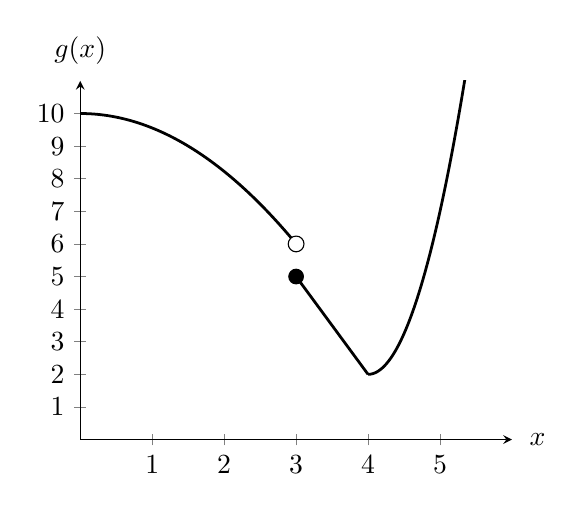
\begin{tikzpicture}
				\begin{axis}[
					scale = .8,
					axis x line = middle,
					axis y line = middle,
	    			every axis y label/.style={at={(ticklabel cs:1.15)}},
	    			ytick = {1,2,...,10},
					y label style={at={(axis description cs:0,1.15)},anchor=north},
	    			ylabel = {\(g(x)\)},
	    			ymin = 0, ymax = 11,
    				every axis x label/.style= {at ={(ticklabel cs:1)}},
    				xtick = {1,2,3,4,5},
    				x label style={at={(axis description cs:1.1,0)},anchor=east},
    				xlabel = {\(x\)},
    				xmin = 0, xmax = 6			
				]
					\addplot [line width=1pt,smooth,samples=100,domain=0.:2.93] {(-.444)*x^2 + 10}; % plots first piece of function
					\coordinate (circle1) at (3,6);
					\addplot[line width = 1pt, smooth, samples = 100, domain = 3.0:4.0] {-3.*x + 14.}; %plot second piece
					\coordinate (circle2) at (3,5);
					\addplot[->,line width = 1pt, smooth, samples = 100, domain = 4.0:6.0] {5*(x - 4)^2 + 2}; %plot third piece
				\end{axis}
				\fill[white] (circle1) circle (.1);
				\draw (circle1) circle (.1);
				\fill (circle2) circle (.1);
			\end{tikzpicture}
			\end{minipage}\hspace{20pt}
			\begin{minipage}{.45\textwidth}
				\begin{multicols*}{2}
					\begin{enumerate}[(a)]
						\setlength\itemsep{.75in}
						\item \(\ds \lim_{x\to 4^-} g(x)=\)     
						\item \(\ds \lim_{x\to 4^+} g(x)=\)     
						\item \(\ds \lim_{x\to 4} g(x)=\) 
							\columnbreak  
						\item \(\ds \lim_{x\to 3^-} g(x)=\)     
						\item \(\ds \lim_{x\to 3^+} g(x)=\)     
						\item \(\ds \lim_{x\to 3} g(x)=\)   
							\raggedcolumns
					\end{enumerate}
				\end{multicols*}
			\end{minipage}
			\end{center}
		\end{ex}
			\vs{1}
			
		\begin{ex}
			Let \(f(x) = \dfrac{|x-3|}{x^2-9}\)
			\begin{enumerate}[(a)]
				\item Find \(\ds \lim_{x\to 3^-} f(x)\)
					\vs{1}
					
				\item Find \(\ds \lim_{x\to 3^+} f(x)\)
					\vs{1}
					\newpage
					
				\item Write a conclusion about \(\ds \lim_{x\to 3} f(x)\).
					\vs{1}
			\end{enumerate}
		\end{ex}
			
		\begin{ex}
			Examine the limit behavior of the function \(r(p) = \dfrac{p^2-64}{p+8}\) at \(p = -8\).  Record your answers will full decimal accuracy, and round your final answer to the thousandths place, if necessary.\\
			\begin{center}
				\begin{minipage}{.45\textwidth}
					\tabulinesep=1mm
					\begin{tabu}{|X[c]|X[1.5,c]|}\hline
						\(p\) 						& \(r(p)\) \\ \hline
												& \\
						\(-8.1\)					& \\ 
												& \\ \hline
												& \\
						\(-8.01\)	& \\
												& \\ \hline 
												& \\
						\(-8.001\)	& \\ 
												& \\ \hline
												& \\ 
						\(-8.0001\)	& \\ 
												& \\ \hline
												& \\
						\(-8.00001\)	&\\
												&\\ \hline\hline
												&\\
						\(\ds \lim_{p\to -8^-}r(p)  =\) & \\
												&\\ \hline
					\end{tabu}
				\end{minipage}
				\begin{minipage}{.45\textwidth}
					\tabulinesep=1mm
					\begin{tabu}{|X[c]|X[1.5,c]|}\hline
						\(p\) 		& \(r(p)\) \\ \hline
								& \\
						\(-7.9\)		& \\ 
								& \\ \hline
								& \\
						\(-7.99\)	& \\
								& \\ \hline 
								& \\
						\(-7.999\)	& \\ 
								& \\ \hline
								& \\ 
						\(-7.9999\)	& \\ 
								& \\ \hline
								& \\
						\(-7.99999\)	&\\
								&\\ \hline\hline
								&\\
						\(\ds \lim_{p\to -8^+}r(p) =\) & \\
								&\\ \hline
					\end{tabu}
				\end{minipage}
					\vs{.5}
				\[\lim_{p\to -8}r(p)= \blank{3}\]
					\vs{.25}
			\end{center}					
		\end{ex}
			\newpage
			
		\begin{ex}
			Sketch the graph of a function which has the following properties:
			\begin{itemize}
				\item \(\ds \lim_{x\to 2} f(x) =1 \)
				\item \(\ds \lim_{x\to 4^-} f(x) = 3\)
				\item \(\ds \lim_{x\to 4^+} f(x) = 6 \)
				\item \(f(4)\) is not defined
			\end{itemize}
		\end{ex}
			\vs{1}
			
	\subsubsection*{Infinite Limits}
		\begin{ex}
			Estimate \(\ds \lim_{x\to 0} -\dfrac{1}{x^2}\).
			\begin{center}
				\begin{minipage}{.45\textwidth}
					\tabulinesep=1mm
					\begin{tabu}{|X[c]|X[1.5,c]|}\hline
						\(x\) 						& \(-\dfrac{1}{x^2}\) \\ \hline
												& \\
						\(-0.1\)					& \\ 
												& \\ \hline
												& \\
						\(-0.01\)	& \\
												& \\ \hline 
												& \\
						\(-0.001\)	& \\ 
												& \\ \hline
												& \\ 
						\(-0.0001\)	& \\ 
												& \\ \hline
												& \\
						\(-0.00001\)	&\\
												&\\ \hline\hline
												&\\
						\(\ds \lim_{x\to 0^-}\lrpar{-\dfrac{1}{x^2}} =\) & \\
												&\\ \hline
					\end{tabu}
				\end{minipage}
				\begin{minipage}{.45\textwidth}
					\tabulinesep=1mm
					\begin{tabu}{|X[c]|X[1.5,c]|}\hline
						\(x\) 						& \(-\dfrac{1}{x^2}\) \\ \hline
												& \\
						\(0.1\)					& \\ 
												& \\ \hline
												& \\
						\(0.01\)	& \\
												& \\ \hline 
												& \\
						\(0.001\)	& \\ 
												& \\ \hline
												& \\ 
						\(0.0001\)	& \\ 
												& \\ \hline
												& \\
						\(0.00001\)	&\\
												&\\ \hline\hline
												&\\
						\(\ds \lim_{x\to 0^+}\lrpar{-\dfrac{1}{x^2}} =\) & \\
												&\\ \hline
					\end{tabu}
				\end{minipage}
					\vs{.25}
				\[\lim_{x\to 0}\lrpar{-\dfrac{1}{x^2}}= \blank{3}\]
					\vs{.25}
			\end{center}	
		\end{ex}		
			\vs{.25}
			\newpage
			
		\begin{rmk}[Notation]
			\\[25pt]
		\end{rmk}
			
		\begin{defn}[Intuitive Definition of an Infinite Limit]
			Let \(f\) be a function defined on both sides of \(a\), except possibly at \(a\) itself.  If the values of \(f(x)\) can be made arbitrarily large, by taking \(x\) sufficiently close to \(a\) (but not equal to \(a\)).  We denote this as\newline\\[100pt]
			
			If the values can be made arbitrarily negative, we denote this as\\[75pt]
			One-sided limits are defined similarly.
		\end{defn}
			\newpage
			
		\begin{ex}
			Sketch an example of each of the following:\\[5pt]
			%\begin{center}
			\begin{minipage}{\textwidth}
				\begin{enumerate}[(a)]
				\setlength\itemsep{2in}
					\begin{multicols*}{2}
						\item \(\ds \lim_{x\to a^-} f(x) = \infty\)
							 
						\item \(\ds \lim_{x\to a^+} f(x) = \infty\)
							 
						\item \(\ds \lim_{x\to a} f(x) = \infty\)
							\columnbreak
							
						\item \(\ds \lim_{x\to a^-} f(x) = -\infty\)
							 
						\item \(\ds \lim_{x\to a^+} f(x) = -\infty\)
							 
						\item \(\ds \lim_{x\to a} f(x) = -\infty\)
							\raggedcolumns									 
					\end{multicols*}
				\end{enumerate}
			\end{minipage}
			%\end{center}
		\end{ex}
			\vs{1}
		
			
		\begin{defn}[Vertical Asymptote]
			The vertical line \(x = a\) is called a \textbf{vertical asymptote} of the curve \(y = f(x)\) if at least one of the following statements is true:\\[75pt]
		\end{defn}
			\newpage
			
		\begin{rmk}[Identifying Vertical Asymptotes, Algebraically]
			A vertical asymptote for a function will occur at every non-removable factor of zero in the denominator.
		\end{rmk}
		
		\begin{ex}
			The function \(k(x) = \dfrac{4x}{x-6}\) has a vertical asymptote at \(x = 6\). Why?
		\end{ex}
			\vs{1}
			
		\begin{ex}
			Find the vertical asymptotes for the function \(f(x) = \dfrac{4x(x-6)}{(x-6)(x^2-3)}\).
		\end{ex}
			\vs{1}
			\newpage
				
	\subsection*{After Class Practice}
		\begin{ex}
			In the theory of relativity, the mass of a particle with velocity \(v\) is given by \(m = \dfrac{m_0}{\sqrt{1-v^2/c^2}}\), where \(m_0\) is the mass of the particle at rest and \(c\) is the speed of light.  What happens as \(v\to c^-\)?
		\end{ex}
			\vs{1}
			
		\begin{ex}
			For any non-zero number \(a\), determine the value of \(\ds \lim_{a\to 0^+} \dfrac{1}{a}\cos \lrpar{\dfrac{\pi}{a}}\).
		\end{ex}
			\vs{1}
			
		\begin{ex}
			Determine the value, if it exists, of \(\ds \lim_{x\to 0} \dfrac{5}{1-e^{1/x}}\)
		\end{ex}
			\vs{1}
	
\clearpage
\end{document}